\documentclass[11pt]{article}
\usepackage[english]{babel}
\usepackage{bm}       % Required for bold math symbols
\usepackage{comment}
\usepackage{booktabs}
\usepackage{subcaption}
\usepackage{siunitx}
\usepackage{enumitem}
\usepackage[a4paper,top=2cm,bottom=2cm,left=2cm,right=2cm]{geometry}
\usepackage{amsmath}
\usepackage{graphicx}
\usepackage[colorlinks=true, allcolors=blue]{hyperref}
\captionsetup{font=footnotesize} % can also use \scriptsize
\usepackage{wrapfig}


% Adjust section title font sizes
\usepackage{titlesec}
%\titleformat*{\section}{\normalsize\bfseries}
%\titleformat*{\subsection}{\small\bfseries}
%\titleformat*{\subsubsection}{\small\bfseries}

\titlespacing*{\section}{0pt}{1ex}{0.5ex}
\titlespacing*{\subsection}{0pt}{1ex}{0.5ex}
\titlespacing*{\subsubsection}{0pt}{0.5ex}{0.5ex}

% Reduce space above and below figures
\setlength{\abovecaptionskip}{3pt}
\setlength{\belowcaptionskip}{0pt}
\setlength{\intextsep}{5pt} % Adjust this value as needed

\title{AS37: The Hubble diagram for type Ia supernovae}
\author{Candidate number: 1054940}

\begin{document}
\maketitle

%-------------------------------------------------------------------

\begin{abstract}
This report presents how we can use the "Hubble diagram" of a sample of 115 type Ia supernovae to show that the universe is expanding. We also show that the data is inconsistent with a flat universe. By combining this data with WMAP data we can also show that the universe expantion is accelerating. 
\end{abstract}

%-------------------------------------------------------------------

\section{Introduction}
In this report we show how type Ia supernovae can be used as "standard candles", since we predict they explode at roughly the same mass, with the same brightness. This allows us to calculate the distance to the star. The speed of these stars relative to Earth is extracted from the red-shift of the light emitted caused by the Doppler Effect. The plot of the speed (or redness) versus time is called a Hubble diagram, after Edwin Hubble, who discovered that there is a linear dependence between the distance to a star and its velocity. 

The data we are analysing consists of the measured redshift and brightness value and its error for 115 supernovae from the "Supernovae Legacy Survey" \cite{SN_legacy_survey}. 


\section{Methods}
\subsection{Friedmann equation}
In this experiment we assume that the universe is uniform and isotropic \cite{AS37_lab_script}, which allows us to write the Friedmann equation: 
\begin{equation}
	H^2(a) = \left( \frac{\dot{a}}{a} \right)^2 = \frac{8 \pi G \rho}{3} - \frac{kc^2}{a^2} + \frac{\Lambda}{3}
	\label{eq:Friedmann}
\end{equation}
where $H(a)$ is the hubble parameter, $a$ is the scale factor, which is defined as 1 at the present time, $\rho$ is the density (due to matter and radiation), $k$ defines the geometry of the space ($k=0$ for a flat universe), and $\Lambda$ is the cosmological constant. We devide equation \eqref{eq:Friedmann} by $H^2$ to find the simplified relation: 
\begin{equation}
	1 = \Omega_M +\Omega_k + \Omega_\Lambda
	\label{eq:main}
\end{equation}

\subsection{Flat universe}
It can be easily seen that if the universe is flat ($k = 0$), meaning that Euclidian geometry applies, or equivalently the angles of any triangle with the sides defined by light rays add up to $180^\circ$, then: 
\begin{equation}
	\Omega_M + \Omega_\Lambda = 1
	\label{eq:flat}
\end{equation}

\subsection{Dark energy}
The cosmological constant is a special case of a more general class of models called "dark energy" models. These models are characterised by the equation of state:
\begin{equation}
	P = w \rho c^2
	\label{eq:dark}
\end{equation}
which relates the pressure $P$ to the energy density $\rho c^2$. $w$ is a constant which is $w = -1$ for the special case of the Cosmological Constant. Also, the value $w = 0$ corresponds to normal matter. therefore we shouldn't try to fit $w = 0$ to the data since we are already accounting for normal matter with the $\Omega_M$ term. 

\section{Results}
\subsection{Linear fit}
We start with the simplest model, the one originally proposed by Edwin Hubble, which predicts a linear relation between the speed and distance of the observed stars. Since the apparent brightness of stars will decrease according to the inverse square law $S \propto d^{-2}$, we expect the slope of the linear fit to be $5$. This is because we are measuring brightness on the magnitude scale.
\begin{equation}
	m = -2.5\log_{10}\frac{S}{S_0}
	\label{eq:mag}
\end{equation}
where $m$ is the magnitude and  $S$ is the apparent brightness. Note that due to the minus sign, fainter objects have higher magnitudes. 

We fit the data with a linear $y = a + bx$ fit. We consider the parameter $a$ "uninteresting", meaning that we allow it to vary while fitting for $b$. We find the slope to be: 
\begin{equation}
	b = 5.50^{5.53}_{5.48}
	\label{res:lin}
\end{equation}
The linear fit has a slope clearly different than $5$, which shows that this simple model does not adequately capture the physics at play. In figure \ref{fig:snls} we plot the dataset and the linear fit, together with the $b = 5$ linear fit. 
\begin{figure}[htbp]
	\centering
	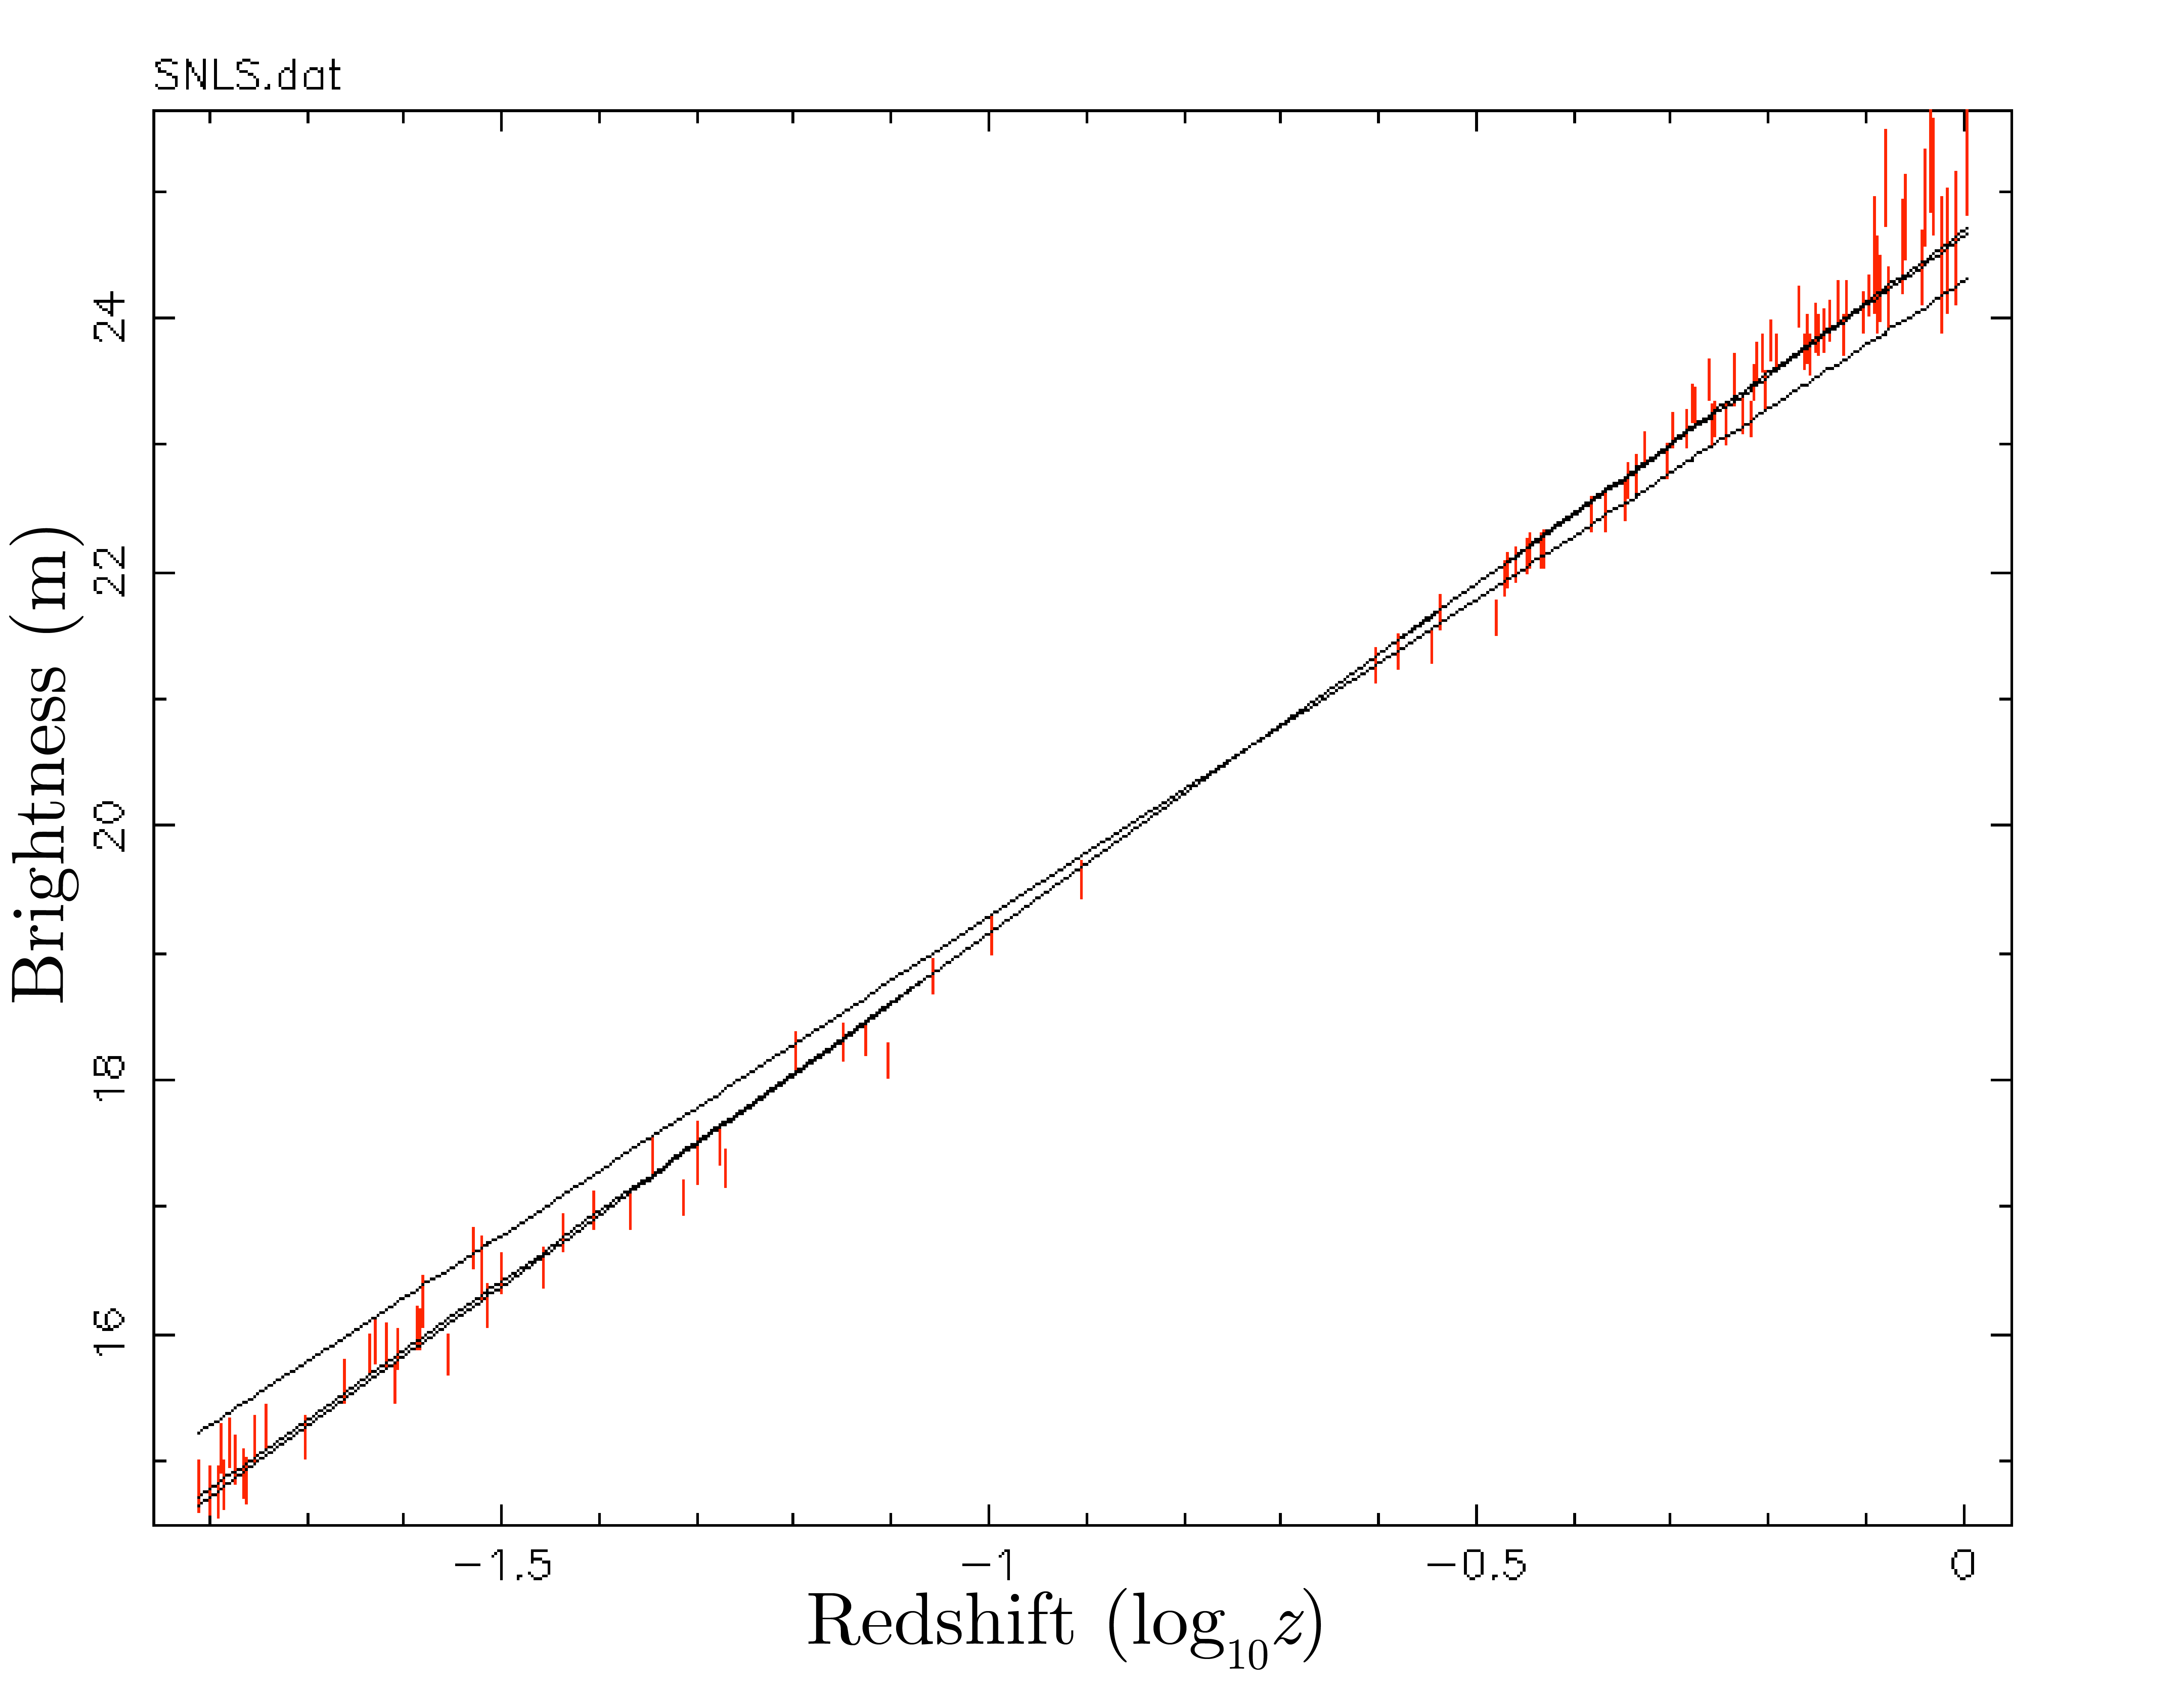
\includegraphics[width=0.8\linewidth]{snls.png}
	\caption{Type Ia supernovae data from the Supernovae Legacy Survey plotted on a Hubble diagram}
	\label{fig:snls}
\end{figure}
We also investigate if this simple model can be a good fit for a range of the data containing only the low redshift datapoints. Analysis of the $\chi^2$ value shows that the linear model breakes down after the first 43 data points, corresponding to a redshift of around $\log_{10}z = -0.95$. 

\subsection{Flat universe model}

\subsection{Non-flat universe models}
\begin{figure}[htbp]
	\centering
	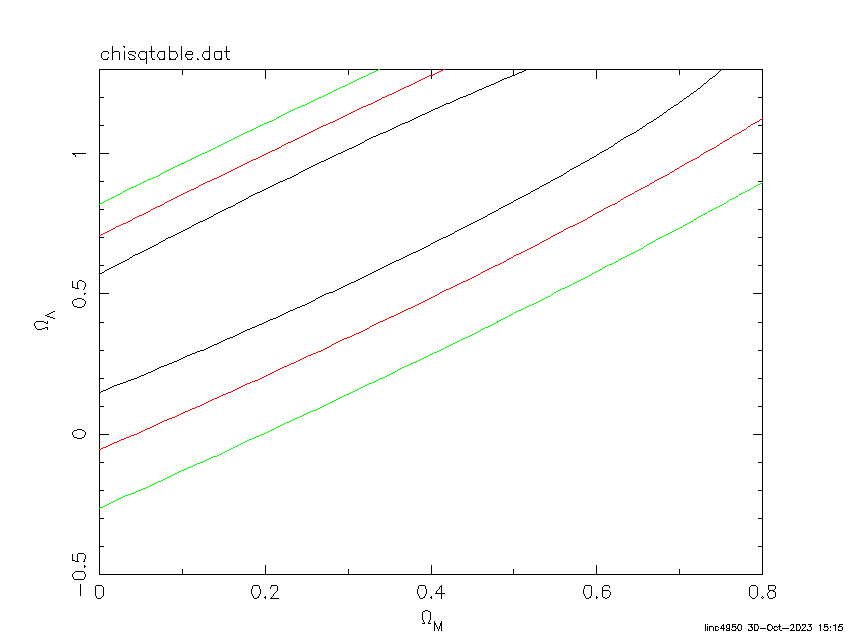
\includegraphics[width=0.8\linewidth]{nonflat.png}
	\caption{Contour plot of the 68\%, 90 \% and 99\% confidence intervals for the cosmological parameters $\Omega_\Lambda$ and $\Omega_M$}
	\label{fig:nonflat}
\end{figure}

\subsection{Dark energy models}
\begin{figure}[htbp]
	\centering
	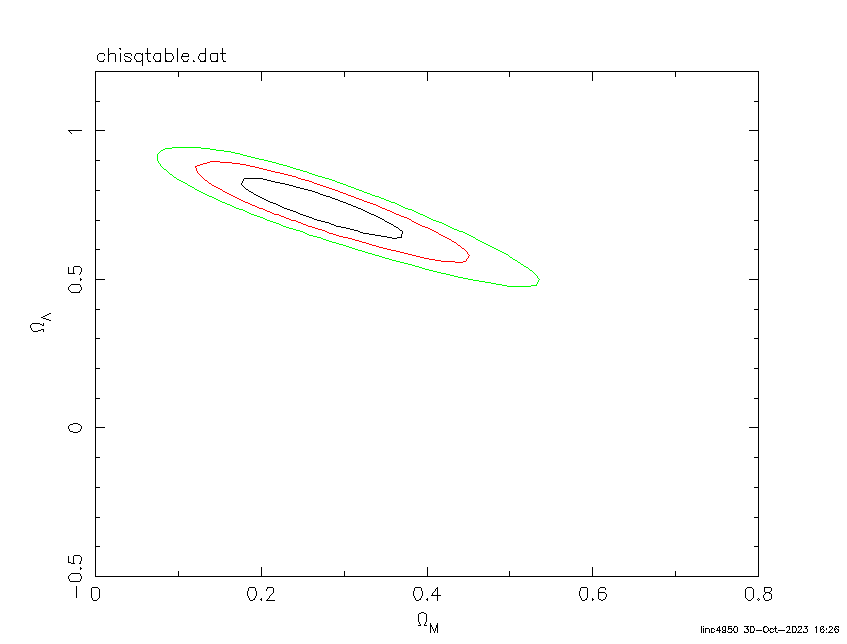
\includegraphics[width=0.8\linewidth]{dark.png}
	\caption{Contour plot of the 68\%, 90 \% and 99\% confidence intervals for the cosmological parameters $\Omega_\Lambda$ and $\Omega_M$}
	\label{fig:dark}
\end{figure}

\section{Conclusions and further work}

\bibliographystyle{plain}
\bibliography{bibliography}

%----------------------------------------------------------------
\newpage

\appendix
\section{some appendix} 
Some text

\end{document}